\part{Wintersemester 2009}
\chapter{Physik (PH)}
\section{2009.10.05}
\subsection{IMG1}
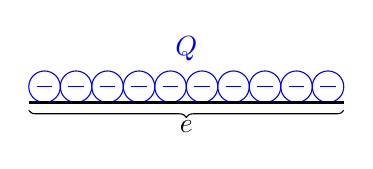
\begin{tikzpicture}
\foreach \x in {0.2,0.6,...,4}
{
	\draw[color=blue] (\x,0.2) circle (0.2);
	\draw[color=blue] (\x-0.1,0.2) -- (\x+0.1,0.2);
}
\draw[thick] (0,0) -- (4,0);
\node[color=blue] at (2,0.4) [above] {$Q$};
\draw decorate [decoration=brace] {(4,-0.1) -- (0,-0.1) node[below,midway] {$e$}};
\end{tikzpicture}

\subsection{IMG2}
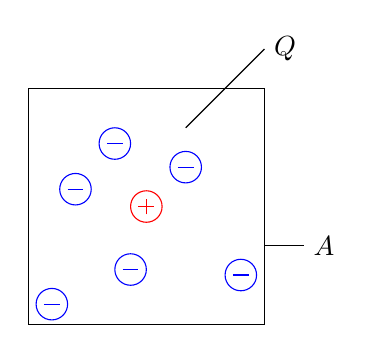
\begin{tikzpicture}
%Negative Ladungen
\foreach \x/\y in
{
0.3/0.26,
0.6/1.72,
2.7/0.63,
2/2,
1.3/0.7,
1.1/2.3
}
{
	\draw[color=blue] (\x,\y) circle (0.2);
	\draw[color=blue] (\x-0.1,\y) -- (\x+0.1,\y);
}

%Positive Ladungen
\foreach \x/\y in
{
1.5/1.5
}
{
	\draw[color=red] (\x,\y) circle (0.2);
	\draw[color=red] (\x-0.1,\y) -- (\x+0.1,\y);
	\draw[color=red] (\x,\y-0.1) -- (\x,\y+0.1);
}

\draw (0,0) rectangle (3,3);

\draw(2,2.5) -- (3,3.5) node[right] {$Q$};
\draw(3,1) -- (3.5,1) node[right] {$A$};

\end{tikzpicture}

\subsection{IMG3}
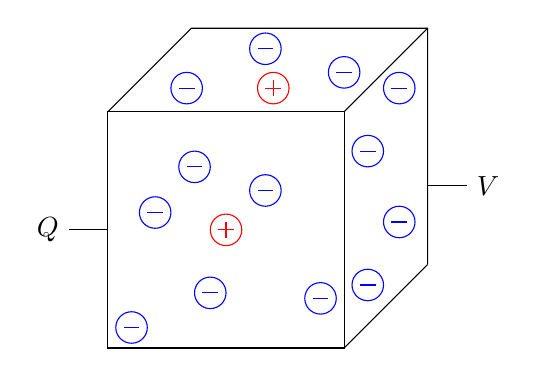
\begin{tikzpicture}
%Negative Ladungen
\foreach \x/\y in
{
0.3/0.26,
0.6/1.72,
2.7/0.63,
2/2,
1.3/0.7,
1.1/2.3,
3.3/2.5,
3.7/3.3,
3.7/1.6,
3.3/0.8,
3/3.5,
1/3.3,
2/3.8
}
{
	\draw[color=blue] (\x,\y) circle (0.2);
	\draw[color=blue] (\x-0.1,\y) -- (\x+0.1,\y);
}

%Positive Ladungen
\foreach \x/\y in
{
1.5/1.5,
2.1/3.3
}
{
	\draw[color=red] (\x,\y) circle (0.2);
	\draw[color=red] (\x-0.1,\y) -- (\x+0.1,\y);
	\draw[color=red] (\x,\y-0.1) -- (\x,\y+0.1);
}

\draw (0,0) rectangle (3,3);
\draw (3,3) -- ++(45:1.5);
\draw (3,0) -- ++(45:1.5);
\draw (0,3) -- ++(45:1.5) -- ++(3,0) -- ++(0,-3);

\draw(0,1.5) -- (-0.5,1.5) node[left] {$Q$};
\draw(3,1) ++(45:1.5) -- ++(0.5,0) node[right] {$V$};

\end{tikzpicture}

\chapter{Mathematik 1 (MA1)}
\section{2009.10.05}
\subsection{IMG1}
/home/hebz0rl/Dokumente/collaboration/Informatik---Hochschule-Regensburg/pictures/pictures/WS2009/MA1/2009.10.05-IMG1.tex

\subsection{IMG2}
/home/hebz0rl/Dokumente/collaboration/Informatik---Hochschule-Regensburg/pictures/pictures/WS2009/MA1/2009.10.05-IMG2.tex

\subsection{IMG3}
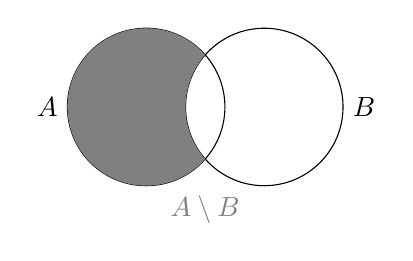
\begin{tikzpicture}
\def\firstcircle{(0,0) circle (1)}
\def\secondcircle{(1.5,0) circle (1)}

\draw \firstcircle;
\draw \secondcircle;

\node at (-1,0) [left] {$A$};
\node at (2.5,0) [right] {$B$};

\begin{scope}[even odd rule]% first circle without the second
\clip \secondcircle (-1,1) rectangle (2.5,-1);
\fill[gray] \firstcircle;
\end{scope}

\node[color=gray] at (0.75,-1) [below] {$A \setminus B$};
\end{tikzpicture}


\subsection{IMG4}
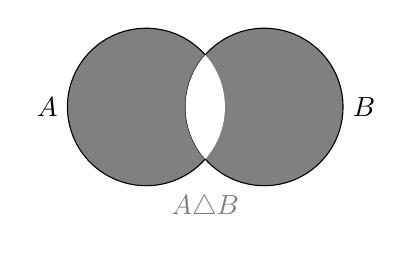
\begin{tikzpicture}
\def\firstcircle{(0,0) circle (1)}
\def\secondcircle{(1.5,0) circle (1)}

\draw[fill=gray] \firstcircle;
\draw[fill=gray] \secondcircle;

\node at (-1,0) [left] {$A$};
\node at (2.5,0) [right] {$B$};

\begin{scope}
\clip \firstcircle;
\fill[white] \secondcircle;
\end{scope}

\node[color=gray] at (0.75,-1) [below] {$A \triangle B$};
\end{tikzpicture}


\subsection{IMG5}
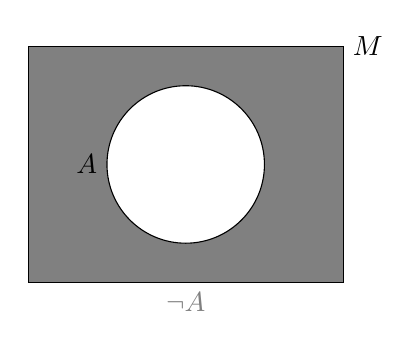
\begin{tikzpicture}
\def\firstcircle{(0,0) circle (1)}

\draw[fill=gray] (-2,-1.5) rectangle (2,1.5) node[right] {$M$};
\draw[fill=white] \firstcircle;

\node at (-1,0) [left] {$A$};

\node[color=gray] at (0,-1.5) [below] {$\neg A$};
\end{tikzpicture}


\section{2009.10.07}
\subsection{IMG1}
/home/hebz0rl/Dokumente/collaboration/Informatik---Hochschule-Regensburg/pictures/pictures/WS2009/MA1/2009.10.07-IMG1.tex

\subsection{IMG2}
/home/hebz0rl/Dokumente/collaboration/Informatik---Hochschule-Regensburg/pictures/pictures/WS2009/MA1/2009.10.07-IMG2.tex

\subsection{IMG3}
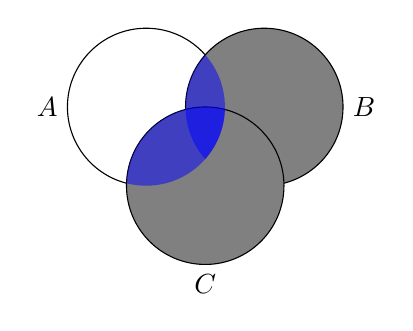
\begin{tikzpicture}
\def\firstcircle{(0,0) circle (1)}
\def\secondcircle{(1.5,0) circle (1)}
\def\thirdcircle{(0.75,-1) circle (1)}

\node at (-1,0) [left] {$A$};
\node at (2.5,0) [right] {$B$};
\node at (0.75,-2) [below] {$C$};

\draw \firstcircle;
\draw[fill=gray] \secondcircle;
\draw[fill=gray] \thirdcircle;

\begin{scope}
\clip \firstcircle;
\clip \secondcircle;
\fill[semitransparent,blue] \secondcircle;
\end{scope}
\begin{scope}
\clip \firstcircle;
\clip \thirdcircle;
\fill[semitransparent,blue] \thirdcircle;
\end{scope}
\end{tikzpicture}


\subsection{IMG4}
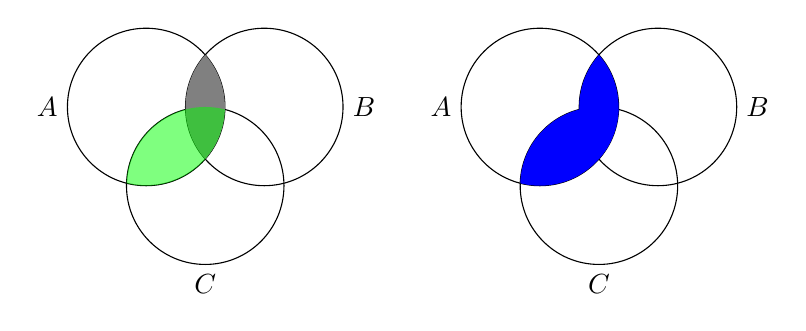
\begin{tikzpicture}
\begin{scope}
\def\firstcircle{(0,0) circle (1)}
\def\secondcircle{(1.5,0) circle (1)}
\def\thirdcircle{(0.75,-1) circle (1)}

\node at (-1,0) [left] {$A$};
\node at (2.5,0) [right] {$B$};
\node at (0.75,-2) [below] {$C$};

\draw \firstcircle;
\draw \secondcircle;
\draw \thirdcircle;

\begin{scope}
\clip \firstcircle;
\clip \secondcircle;
\fill[gray] \secondcircle;
\end{scope}
\begin{scope}
\clip \firstcircle;
\clip \thirdcircle;
\fill[semitransparent,green] \thirdcircle;
\end{scope}
\end{scope}

\node at (3.25,-0.75) {\Large \Ra};

\begin{scope}
\def\firstcircle{(5,0) circle (1)}
\def\secondcircle{(6.5,0) circle (1)}
\def\thirdcircle{(5.75,-1) circle (1)}

\node at (4,0) [left] {$A$};
\node at (7.5,0) [right] {$B$};
\node at (5.75,-2) [below] {$C$};

\draw \firstcircle;
\draw \secondcircle;
\draw \thirdcircle;

\begin{scope}
\clip \firstcircle;
\clip \secondcircle;
\fill[blue] \secondcircle;
\end{scope}
\begin{scope}
\clip \firstcircle;
\clip \thirdcircle;
\fill[blue] \thirdcircle;
\end{scope}
\end{scope}
\end{tikzpicture}


\subsection{IMG5}
/home/hebz0rl/Dokumente/collaboration/Informatik---Hochschule-Regensburg/pictures/pictures/WS2009/MA1/2009.10.07-IMG5.tex

\section{2009.10.15}
\subsection{IMG1}
/home/hebz0rl/Dokumente/collaboration/Informatik---Hochschule-Regensburg/pictures/pictures/WS2009/MA1/2009.10.15-IMG1.tex

\subsection{IMG2}
/home/hebz0rl/Dokumente/collaboration/Informatik---Hochschule-Regensburg/pictures/pictures/WS2009/MA1/2009.10.15-IMG2.tex

\subsection{IMG3}
\begin{tikzpicture}
\node at (0,0) [right] {
$\begin{pmatrix}
w & f & f & f\\
w & w & f & f\\
w & w & f & f
\end{pmatrix}$};

\node at (-0.2,0) [left] {$A$};
\node at (0.2,0.5) [left] {$1$};
\node at (0.2,0) [left] {$2$};
\node at (0.2,-0.5) [left] {$3$};

\node at (1.5,0.75) [above] {$B$};

\node at (0.65,-0.75) [below] {$0$};
\node at (1.25,-0.75) [below] {$2$};
\node at (1.85,-0.75) [below] {$4$};
\node at (2.45,-0.75) [below] {$6$};
\end{tikzpicture}


\subsection{IMG4}
\begin{automat}
\node[state] (2) {$2$};
\node[state, right of=2] (3) {$3$};
\node[state, above right of=2] (1) {$1$};

\path[->] (2) edge (1);
\path[->] (2) edge[loop left] ();

\path[->] (3) edge (1);
\path[->] (3) edge (2);
\path[->] (3) edge[loop right] ();

\path[->] (1) edge[loop right] ();
\end{automat}

